\documentclass[landscape,final,a0paper,fontscale=0.285]{baposter}

\usepackage{calc}
\usepackage{graphicx}
\usepackage{amsmath}
\usepackage{amssymb}
\usepackage{relsize}
\usepackage{multirow}
\usepackage{rotating}
\usepackage{bm}
\usepackage{url}
\usepackage{color}
\usepackage{colortbl}
\usepackage{parcolumns}

\usepackage{graphicx}
\usepackage{multicol}
\usepackage{picture}

%\usepackage{times}
%\usepackage{helvet}
%\usepackage{bookman}
\usepackage{palatino}
\usepackage{xspace}
\usepackage{booktabs}
\usepackage{listings}
\usepackage{algpseudocode}
\usepackage{algorithm}


\newcommand{\captionfont}{\footnotesize}

\graphicspath{{images/}{../images/}}
%\usetikzlibrary{calc}

\newcommand{\SET}[1]  {\ensuremath{\mathcal{#1}}}
\newcommand{\MAT}[1]  {\ensuremath{\boldsymbol{#1}}}
\newcommand{\VEC}[1]  {\ensuremath{\boldsymbol{#1}}}
\newcommand{\Video}{\SET{V}}
\newcommand{\video}{\VEC{f}}
\newcommand{\track}{x}
\newcommand{\Track}{\SET T}
\newcommand{\LMs}{\SET L}
\newcommand{\lm}{l}
\newcommand{\PosE}{\SET P}
\newcommand{\posE}{\VEC p}
\newcommand{\negE}{\VEC n}
\newcommand{\NegE}{\SET N}
\newcommand{\Occluded}{\SET O}
\newcommand{\occluded}{o}

\newcommand{\madden}{\textsc{MADden}\xspace}
\newcommand{\probkb}{\textsc{ProbKB}\xspace}
\newcommand{\camel}{\textsc{CAMeL}\xspace}
\newcommand{\eat}[1]{}


%%%%%%%%%%%%%%%%%%%%%%%%%%%%%%%%%%%%%%%%%%%%%%%%%%%%%%%%%%%%%%%%%%%%%%%%%%%%%%%%
%%%% Some math symbols used in the text
%%%%%%%%%%%%%%%%%%%%%%%%%%%%%%%%%%%%%%%%%%%%%%%%%%%%%%%%%%%%%%%%%%%%%%%%%%%%%%%%

%%%%%%%%%%%%%%%%%%%%%%%%%%%%%%%%%%%%%%%%%%%%%%%%%%%%%%%%%%%%%%%%%%%%%%%%%%%%%%%%
% Multicol Settings
%%%%%%%%%%%%%%%%%%%%%%%%%%%%%%%%%%%%%%%%%%%%%%%%%%%%%%%%%%%%%%%%%%%%%%%%%%%%%%%%
\setlength{\columnsep}{1em}
\setlength{\columnseprule}{0mm}

%%%%%%%%%%%%%%%%%%%%%%%%%%%%%%%%%%%%%%%%%%%%%%%%%%%%%%%%%%%%%%%%%%%%%%%%%%%%%%%%
% Save space in lists. Use this after the opening of the list
%%%%%%%%%%%%%%%%%%%%%%%%%%%%%%%%%%%%%%%%%%%%%%%%%%%%%%%%%%%%%%%%%%%%%%%%%%%%%%%%
\newcommand{\compresslist}{%
\setlength{\itemsep}{1pt}%
\setlength{\parskip}{0pt}%
\setlength{\parsep}{0pt}%
}

\definecolor{lightgray}{rgb}{0.98,0.98,0.98}

\renewcommand{\ttdefault}{pcr}
\lstset{
  language=SQL,
  basicstyle={\footnotesize\ttfamily},
  numbers=none,
  backgroundcolor=\color{lightgray},
  aboveskip=3mm,
  belowskip=3mm,
  showstringspaces=false,
  columns=flexible,
  keywordstyle={\bfseries\color{blue}},
  commentstyle={\color{red}\textit},
  stringstyle=\color{magenta},
  frame=single,
  breaklines=true,
  breakatwhitespace=true,
  tabsize=4
}
%%%%%%%%%%%%%%%%%%%%%%%%%%%%%%%%%%%%%%%%%%%%%%%%%%%%%%%%%%%%%%%%%%%%%%%%%%%%%%
%%% Begin of Document
%%%%%%%%%%%%%%%%%%%%%%%%%%%%%%%%%%%%%%%%%%%%%%%%%%%%%%%%%%%%%%%%%%%%%%%%%%%%%%

\begin{document}
%%%%%%%%%%%%%%%%%%%%%%%%%%%%%%%%%%%%%%%%%%%%%%%%%%%%%%%%%%%%%%%%%%%%%%%%%%%%%%
%%% Here starts the poster
%%%---------------------------------------------------------------------------
%%% Format it to your taste with the options
%%%%%%%%%%%%%%%%%%%%%%%%%%%%%%%%%%%%%%%%%%%%%%%%%%%%%%%%%%%%%%%%%%%%%%%%%%%%%%
% Define some colors

\definecolor{lightblue}{cmyk}{0.83,0.24,0,0.12}
%\definecolor{lightblue}{rgb}{0.145,0.6666,1}

% Draw a video
\newlength{\FSZ}
\newcommand{\drawvideo}[3]{% [0 0.25 0.5 0.75 1 1.25 1.5]
   \noindent\pgfmathsetlength{\FSZ}{\linewidth/#2}
   \begin{tikzpicture}[outer sep=0pt,inner sep=0pt,x=\FSZ,y=\FSZ]
   \draw[color=lightblue!50!black] (0,0) node[outer sep=0pt,inner sep=0pt,text width=\linewidth,minimum height=0] (video) {\noindent#3};
   \path [fill=lightblue!50!black,line width=0pt] 
     (video.north west) rectangle ([yshift=\FSZ] video.north east) 
    \foreach \x in {1,2,...,#2} {
      {[rounded corners=0.6] ($(video.north west)+(-0.7,0.8)+(\x,0)$) rectangle +(0.4,-0.6)}
    }
;
   \path [fill=lightblue!50!black,line width=0pt] 
     ([yshift=-1\FSZ] video.south west) rectangle (video.south east) 
    \foreach \x in {1,2,...,#2} {
      {[rounded corners=0.6] ($(video.south west)+(-0.7,-0.2)+(\x,0)$) rectangle +(0.4,-0.6)}
    }
;
   \foreach \x in {1,...,#1} {
     \draw[color=lightblue!50!black] ([xshift=\x\linewidth/#1] video.north west) -- ([xshift=\x\linewidth/#1] video.south west);
   }
   \foreach \x in {0,#1} {
     \draw[color=lightblue!50!black] ([xshift=\x\linewidth/#1,yshift=1\FSZ] video.north west) -- ([xshift=\x\linewidth/#1,yshift=-1\FSZ] video.south west);
   }
   \end{tikzpicture}
}

\hyphenation{resolution occlusions}
%%
\begin{poster}%
  % Poster Options
  {
  % Show grid to help with alignment
  grid=false,
  % Column spacing
  colspacing=1em,
  % Color style
  bgColorOne=white,
  bgColorTwo=white,
  borderColor=lightblue,
  headerColorOne=black,
  headerColorTwo=lightblue,
  headerFontColor=white,
  boxColorOne=white,
  boxColorTwo=lightblue,
  boxpadding=7px,
  % Format of textbox
  textborder=roundedleft,
  % Format of text header
  eyecatcher=false,
  headerborder=closed,
  headerheight=0.170\textheight,
  %headerheight=0.125\textheight,
%  textfont=\sc, An example of changing the text font
  headershape=roundedright,
  headershade=shadelr,
  headerfont=\Large\bf\textsc, %Sans Serif
  textfont={\setlength{\parindent}{1.5em}},
  boxshade=plain,
%  background=shade-tb,
  background=plain,
  linewidth=2pt
  }
  % Eye Catcher
  {\includegraphics[height=3em]{images/graph_occluded.pdf}}
  % Title
  {\vspace*{.3em}\bf{\underline{ProbKB: Managing Web-Scale Knowledge}}\vspace{0.1em}
      {\newline\Large\underline{CIS6930 LRG ADV DATA ANLY}}\vspace{0.1em}}
  % Authors
  {\textsc{Yang Chen$^{\S}$, Xing Liu$^{\S}$, \\[0.1em]
                    {$^{\S}$\textit{CISE, University of Florida} }}\\[0.1em]
             {\textit{\textcolor{blue} {\{yang,xinliu\} @cise.ufl.edu}}}}
  % University logo
  {% The makebox allows the title to flow into the logo, this is a hack because of the L shaped logo.
    
\includegraphics[height=8.5em]{logo/UF_Signature_Themeline.pdf}
  }\vspace{-3mm}

%%%%%%%%%%%%%%%%%%%%%%%%%%%%%%%%%%%%%%%%%%%%%%%%%%%%%%%%%%%%%%%%%%%%%%%%%%%%%%
%%% Now define the boxes that make up the poster
%%%---------------------------------------------------------------------------
%%% Each box has a name and can be placed absolutely or relatively.
%%% The only inconvenience is that you can only specify a relative position 
%%% towards an already declared box. So if you have a box attached to the 
%%% bottom, one to the top and a third one which should be in between, you 
%%% have to specify the top and bottom boxes before you specify the middle 
%%% box.
%%%%%%%%%%%%%%%%%%%%%%%%%%%%%%%%%%%%%%%%%%%%%%%%%%%%%%%%%%%%%%%%%%%%%%%%%%%%%%
    %
    % A coloured circle useful as a bullet with an adjustably strong filling
    \newcommand{\colouredcircle}{%
      \tikz{\useasboundingbox (-0.2em,-0.32em) rectangle(0.2em,0.32em); \draw[draw=black,fill=lightblue,line width=0.03em] (0,0) circle(0.18em);}}

%%%%%%%%%%%%%%%%%%%%%%%%%%%%%%%%%%%%%%%%%%%%%%%%%%%%%%%%%%%%%%%%%%%%%%%%%%%%%%
  \headerbox{Abstract}{name=myabstract,column=0,row=0}{
%%%%%%%%%%%%%%%%%%%%%%%%%%%%%%%%%%%%%%%%%%%%%%%%%%%%%%%%%%%%%%%%%%%%%%%%%%%%%%
      \newcommand{\compactlist}{\setlength{\itemsep}{0pt} \setlength{\parskip}{0pt} \setlength{\leftskip}{-1em}}
      
ProbKB, a PROBabilistic Knowledge Base constructed from web scale extracted
entities, facts, and rules represented as a Markov logic network (MLN). 
We achieved web scale MLN inference by designing a novel
structured, relational model for MLNs and efficient grounding algorithms that apply rules
in batches. Errors are handled in a principled
and elegant manner to avoid unnecessary resource consumption. The inference task is
delegated to GraphLab, a distributed framework designed specifically for machine learning problems. Our initial experiments show
that our approach has much better scalability
than the state-of-the-art.
    }
    
%%%%%%%%%%%%%%%%%%%%%%%%%%%%%%%%%%%%%%%%%%%%%%%%%%%%%%%%%%%%%%%%%%%%%%%%%%%%%%
  \headerbox{System Overview}{name=myintroduction,column=0,below=myabstract}{
%%%%%%%%%%%%%%%%%%%%%%%%%%%%%%%%%%%%%%%%%%%%%%%%%%%%%%%%%%%%%%%%%%%%%%%%%%%%%%
   \newcommand{\compactlist}{\setlength{\itemsep}{0pt} \setlength{\parskip}{0pt} \setlength{\leftskip}{-1em}}
    \begin{center}
 %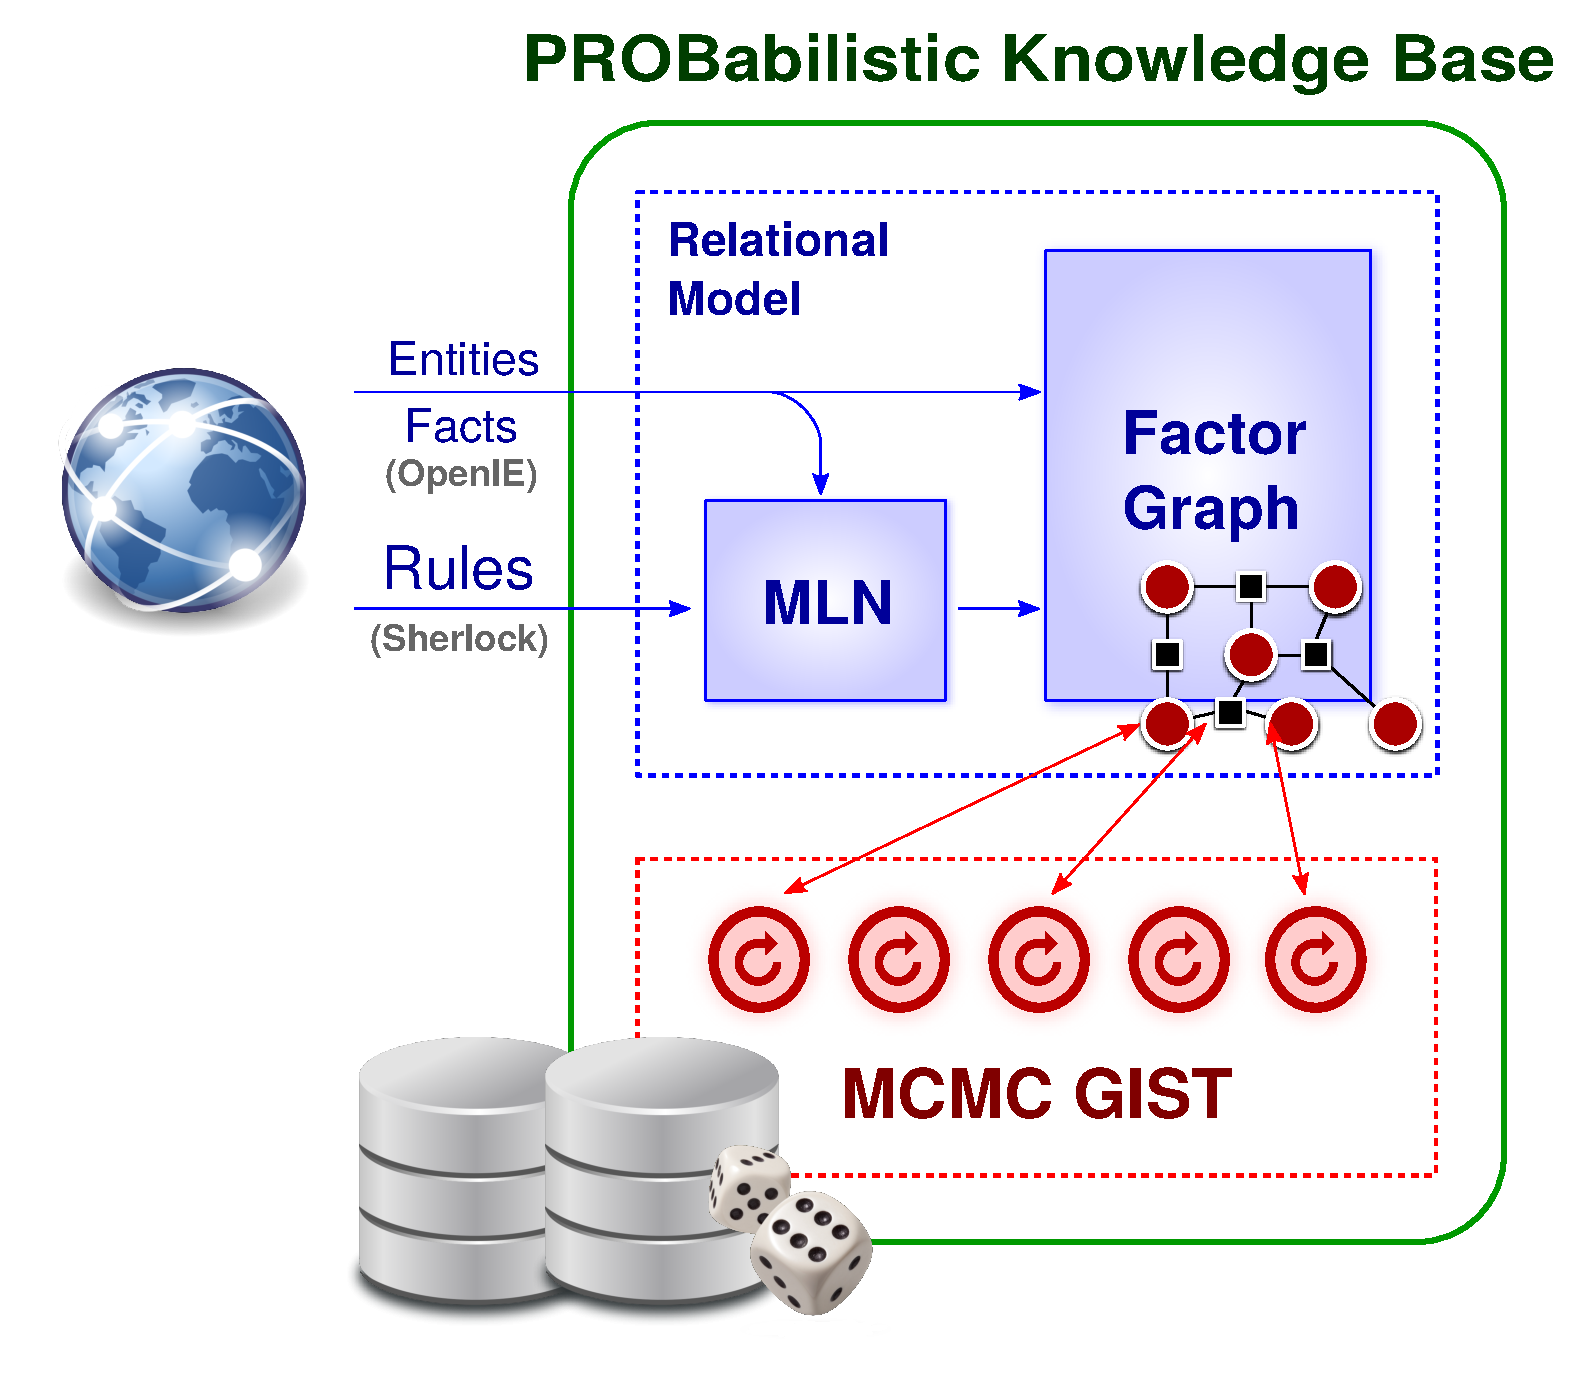
\includegraphics[height=9em]{images/probkbarch.pdf}    
  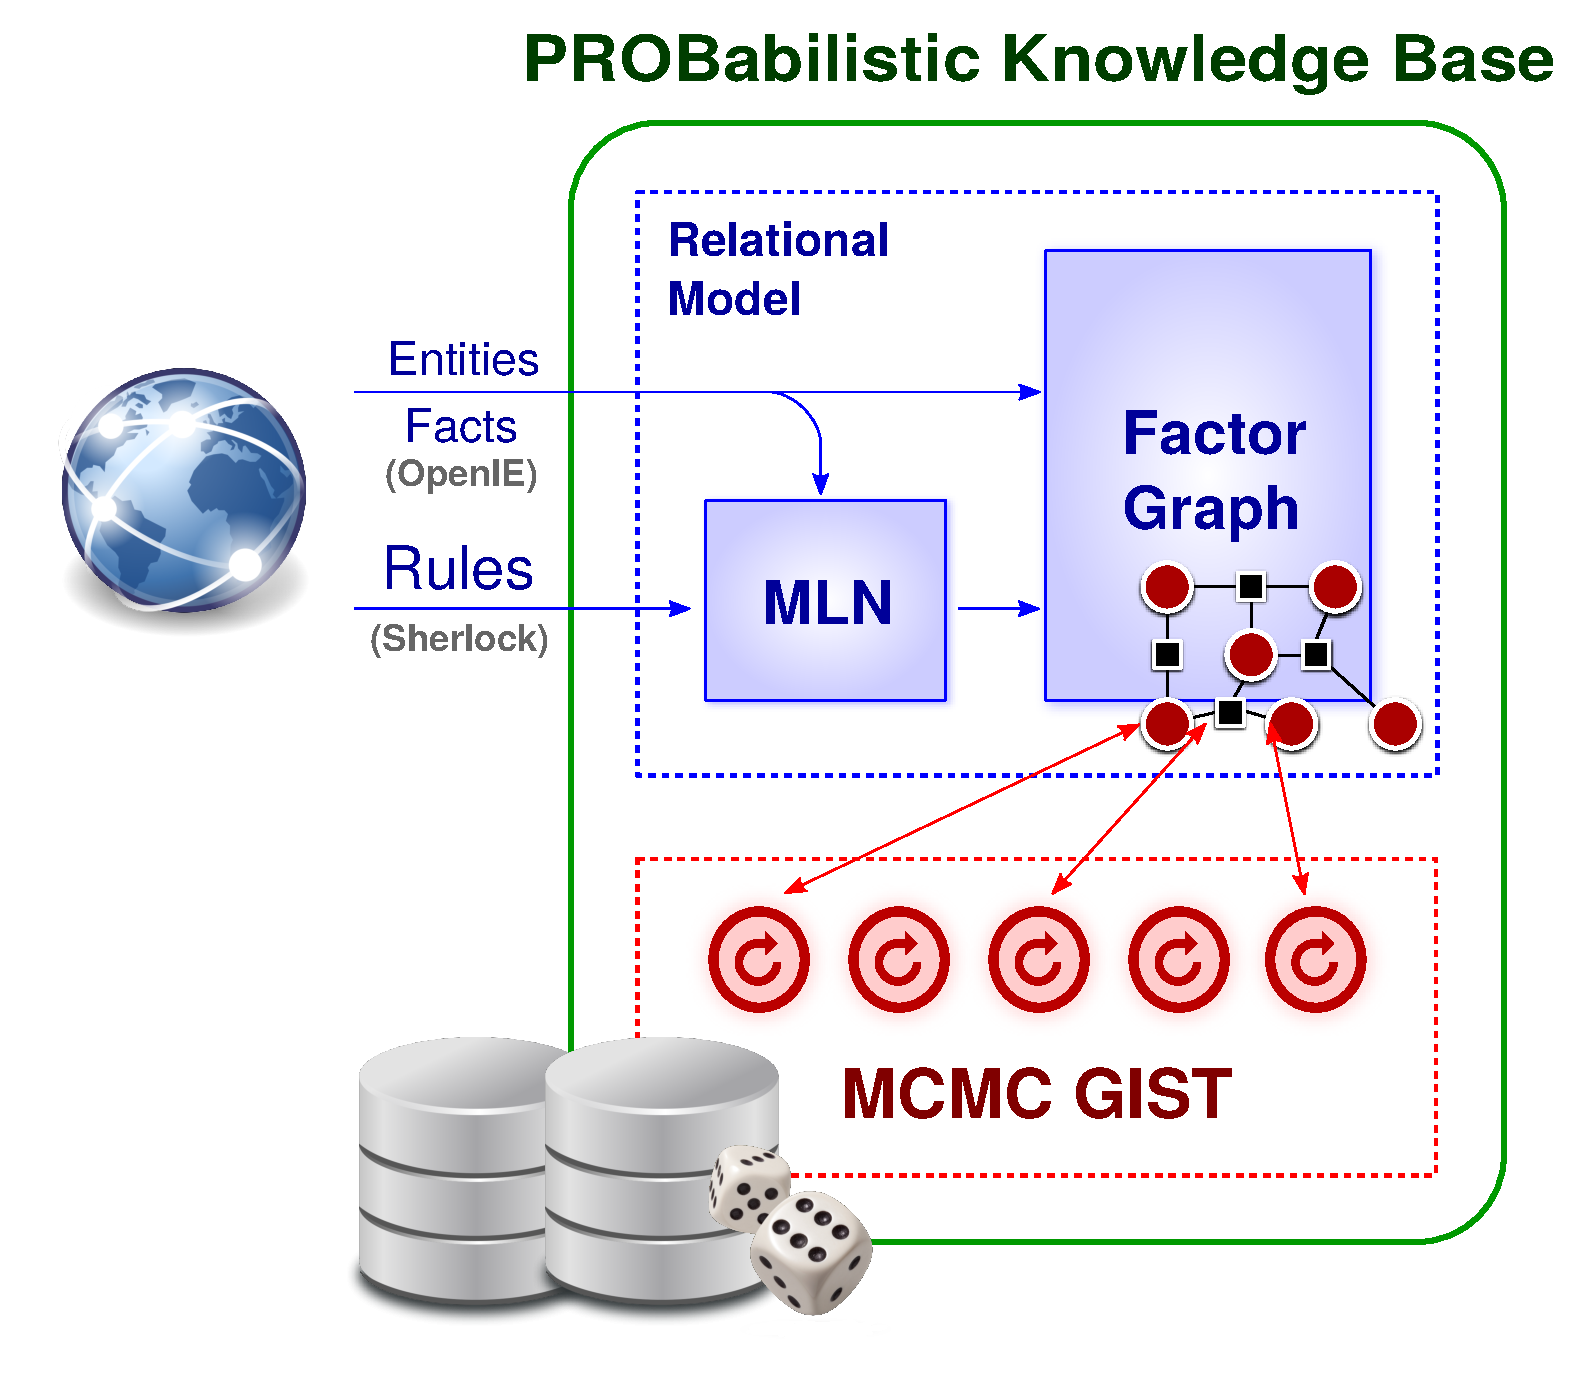
\includegraphics[height=18em]{images/probkbarch.pdf}
    \end{center}
    }

%%%%%%%%%%%%%%%%%%%%%%%%%%%%%%%%%%%%%%%%%%%%%%%%%%%%%%%%%%%%%%%%%%%%%%%%%%%%%%
  \headerbox{\large Challenges and Current Work}{name=challenges,column=0,below=myintroduction}{
%%%%%%%%%%%%%%%%%%%%%%%%%%%%%%%%%%%%%%%%%%%%%%%%%%%%%%%%%%%%%%%%%%%%%%%%%%%%%%
   \newcommand{\compactlist}{\setlength{\itemsep}{0pt} \setlength{\parskip}{0pt} \setlength{\leftskip}{-1em}}
   \begin{itemize}\compactlist
     \item Item 1.
     \item Item 2.
     \item Item 3.
     \item Item 4.
     \item Item 5.
   \end{itemize}
    
    }


 %%%%%%%%%%%%%%%%%%%%%%%%%%%%%%%%%%%%%%%%%%%%%%%%%%%%%%%%%%%%%%%%%%%%%%%%%%%%%%
 % \headerbox{Acknowledgements}{name=myacknowledgements,column=0,below=challenges}{
%%%%%%%%%%%%%%%%%%%%%%%%%%%%%%%%%%%%%%%%%%%%%%%%%%%%%%%%%%%%%%%%%%%%%%%%%%%%%%
  %      \includegraphics[width=0.85\linewidth]{T-labs-Drawing-1} 
  %    \newcommand{\compactlist}{\setlength{\itemsep}{0pt} \setlength{\parskip}{0pt} \setlength{\leftskip}{-1em}}
    
%Acknowledgements including AWS credits.

    %      }

%%%%%%%%%%%%%%%%%%%%%%%%%%%%%%%%%%%%%%%%%%%%%%%%%%%%%%%%%%%%%%%%%%%%%%%%%%%%%%
\headerbox{Relational MLN Model}{name=myourapproach,column=1,span=3,row=0}{
%%%%%%%%%%%%%%%%%%%%%%%%%%%%%%%%%%%%%%%%%%%%%%%%%%%%%%%%%%%%%%%%%%%%%%%%%%%%%%
  \newcommand{\compactlist}{\setlength{\itemsep}{0pt} \setlength{\parskip}{0pt} \setlength{\leftskip}{-1em}}

  \begin{itemize}\compactlist
     \item Put entities, facts, and rules into the database, so that the rules are applied in batches, and wrapped the grounding logic into stored procedures.
     \item Considered Horn clauses only.Identify six rules pattern in SHERLOCK rules.Each rule type i has a table Mi recording the predicates involved in the rules of that type.
     \item Another table R for relationships. For each relationship p(x, y) that is stated in the text corpus, we have a tuple (p, x, y) in R. 

   \end{itemize}
}

%%%%%%%%%%%%%%%%%%%%%%%%%%%%%%%%%%%%%%%%%%%%%%%%%%%%%%%%%%%%%%%%%%%%%%%%%%%%%%
\headerbox{Grounding}{name=myapproxstrmatch,column=1,span=2,below=myourapproach} {
%%%%%%%%%%%%%%%%%%%%%%%%%%%%%%%%%%%%%%%%%%%%%%%%%%%%%%%%%%%%%%%%%%%%%%%%%%%%%%
 
  \newcommand{\compactlist}{\setlength{\itemsep}{0pt} \setlength{\parskip}{0pt} \setlength{\leftskip}{-1em}}
  
\begin{itemize}\compactlist
     \item Used lazy inference and adopted a one-step look-ahead strategy: assume all
atoms are inactive and compute active clauses. activate the atoms in the grounding result and recompute active clauses. 
     


     \item Assume rules of type 3 are stored in table M3 (p, q, r), and relationships p(x, y) are stored in R(p, x, y), then the
following SQL query computes atoms that are activated during the grounding process ,this process is repeated until convergence, resulting
in an active closure. The following SQL query then
computes active clauses given the active atoms:

  
 \begin{lstlisting}[language=SQL]^^J
SELECT DISTINCT ^^J
R1.id AS id1, R2.id AS id2, R3.id AS id3 ^^J
FROM M3 JOIN R R ON M3.p = R.p ^^J
JOIN R R1 ON M3.q = R1.p ^^J
JOIN R R2 ON M3.r = R2.p ^^J
WHERE R.x = R1.x AND R.y = R2.x AND R1.y = R2.y ^^J 
\end{lstlisting}




   \item The result of grounding is a factor graph (Markov network). This graph encodes a probability distribution
over its variable nodes, which can be used to answer
user queries. We use TUFFY as comparison point. We tried to run ProbKB using the ReVerb-
Sherlock dataset and measured the grounding time in 85 seconds whereas TUFFY crashes in this step.


   \end{itemize}


}
%%%%%%%%%%%%%%%%%%%%%%%%%%%%%%%%%%%%%%%%%%%%%%%%%%%%%%%%%%%%%%%%%%%%%%%%%%%%%%%
%%%%%%%%%%%%%%%%%%%%%%%%%%%%%%%%%%%%%%%%%%%%%%%%%%%%%%%%%%%%%%%%%%%%%%%%%%%%%%%
\headerbox{Knowledge Integrity}{name=mycer1,column=3,span=1,below=myourapproach} {
  \newcommand{\compactlist}{\setlength{\itemsep}{0pt} \setlength{\parskip}{0pt} \setlength{\leftskip}{-1em}}
\begin{itemize}\compactlist
\item Few common error patterns (ambiguity, meaningless relations, etc) that might affect learning quality. We use robust semi-naive evalution to emphasize the fact that inferences only occur among most correst facts and errors are unlikely to arise.
    
\begin{algorithmic}
\State $candidates \gets all facts $
\State $beliefs \gets promote( \varnothing ,candidates) $
\State $delta = \varnothing $
\Repeat 
\State $promoter  \gets infer(beliefs,delta) $
\State $beliefs  \gets beliefs \cup delta $
\State $delta \gets \varnothing $
\Until 

\end{algorithmic}
  

\end{itemize}
}

%%%%%%%%%%%%%%%%%%%%%%%%%%%%%%%%%%%%%%%%%%%%%%%%%%%%%%%%%%%%%%%%%%%%%%%%%%%%%%%
%%%%%%%%%%%%%%%%%%%%%%%%%%%%%%%%%%%%%%%%%%%%%%%%%%%%%%%%%%%%%%%%%%%%%%%%%%%%%%%
\headerbox{Inference}{name=mycer,column=1,span=3,below=myapproxstrmatch} {
  \newcommand{\compactlist}{\setlength{\itemsep}{0pt} \setlength{\parskip}{0pt} \setlength{\leftskip}{-1em}}
   
 \begin{multicols}{2}

\begin{itemize}\compactlist
     \item Use MCMC algorithm to do the marginal inference in MLN. The results are the marginal probablity of grounding facts.

     \item Our first approach is using Metropolis–Hastings algorithm with Datapath as our parallel engine. Partition the graph to subgraphs and runs the algorithm on each of them. We found this approach could break the Markov Logic Network if a factor is accross several subgraphs.  

     \item Our second approach is to use a write lock on each variable on the factor graph and random walk on the whole graph instead of partition the graph, and collecting samples in parallel.  
    
     \item Because of performance and accuracy issue, Our lattest approach is that runs Gibbs sampling using GraphLab as our parallel engine.
     \item We sampled a subset with 700 facts and compared the time spent on generating 200 joint samples for ProbKB and Tuffy. It took ProbKB 0.47 minute to complete the inference whereas TUFFY used 55 minutes.

     
   \end{itemize}

 \begin{multicols}{2}
\begin{center}
 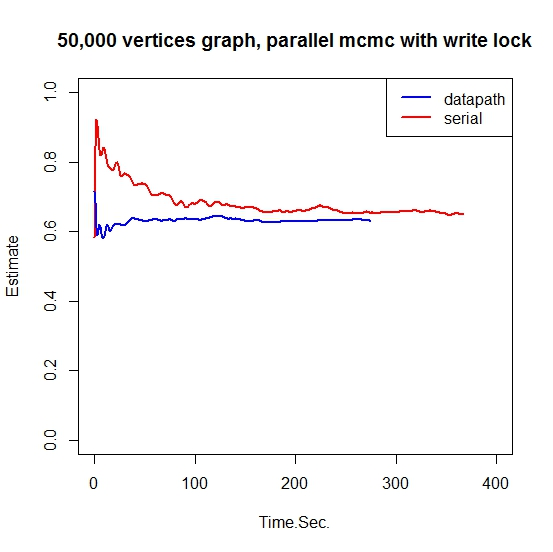
\includegraphics[height=9em]{images/R1.jpeg}  
  \end{center} 
\begin{center}
 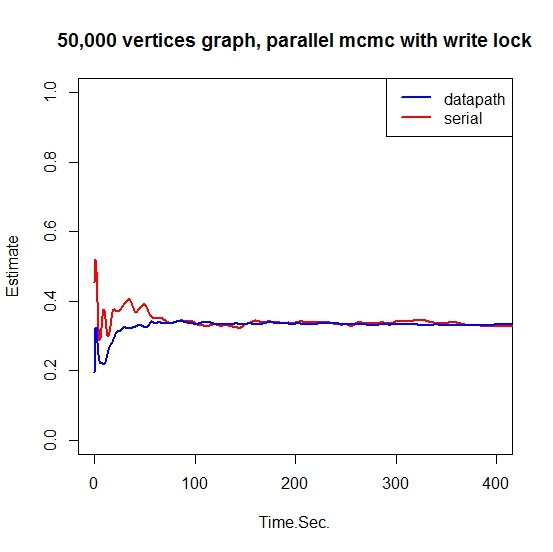
\includegraphics[height=9em]{images/R3.jpeg}  
  \end{center} 
 \end{multicols}{2}


 \end{multicols}{2}


}
    
    
\end{poster}

\end{document}
